%\VignetteIndexEntry{Visualize and RNA-seq data normalization with the "NVT" package}
%\VignettePackage{NVT}
%\VignetteEngine{knitr::knitr}

% To compile this document
% library('knitr'); rm(list=ls()); knit('NVT.Rnw')

\documentclass[11pt]{article}\usepackage[]{graphicx}\usepackage[]{color}
%% maxwidth is the original width if it is less than linewidth
%% otherwise use linewidth (to make sure the graphics do not exceed the margin)
\makeatletter
\def\maxwidth{ %
  \ifdim\Gin@nat@width>\linewidth
    \linewidth
  \else
    \Gin@nat@width
  \fi
}
\makeatother

\definecolor{fgcolor}{rgb}{0.345, 0.345, 0.345}
\newcommand{\hlnum}[1]{\textcolor[rgb]{0.686,0.059,0.569}{#1}}%
\newcommand{\hlstr}[1]{\textcolor[rgb]{0.192,0.494,0.8}{#1}}%
\newcommand{\hlcom}[1]{\textcolor[rgb]{0.678,0.584,0.686}{\textit{#1}}}%
\newcommand{\hlopt}[1]{\textcolor[rgb]{0,0,0}{#1}}%
\newcommand{\hlstd}[1]{\textcolor[rgb]{0.345,0.345,0.345}{#1}}%
\newcommand{\hlkwa}[1]{\textcolor[rgb]{0.161,0.373,0.58}{\textbf{#1}}}%
\newcommand{\hlkwb}[1]{\textcolor[rgb]{0.69,0.353,0.396}{#1}}%
\newcommand{\hlkwc}[1]{\textcolor[rgb]{0.333,0.667,0.333}{#1}}%
\newcommand{\hlkwd}[1]{\textcolor[rgb]{0.737,0.353,0.396}{\textbf{#1}}}%

\usepackage{framed}
\makeatletter
\newenvironment{kframe}{%
 \def\at@end@of@kframe{}%
 \ifinner\ifhmode%
  \def\at@end@of@kframe{\end{minipage}}%
  \begin{minipage}{\columnwidth}%
 \fi\fi%
 \def\FrameCommand##1{\hskip\@totalleftmargin \hskip-\fboxsep
 \colorbox{shadecolor}{##1}\hskip-\fboxsep
     % There is no \\@totalrightmargin, so:
     \hskip-\linewidth \hskip-\@totalleftmargin \hskip\columnwidth}%
 \MakeFramed {\advance\hsize-\width
   \@totalleftmargin\z@ \linewidth\hsize
   \@setminipage}}%
 {\par\unskip\endMakeFramed%
 \at@end@of@kframe}
\makeatother

\definecolor{shadecolor}{rgb}{.97, .97, .97}
\definecolor{messagecolor}{rgb}{0, 0, 0}
\definecolor{warningcolor}{rgb}{1, 0, 1}
\definecolor{errorcolor}{rgb}{1, 0, 0}
\newenvironment{knitrout}{}{} % an empty environment to be redefined in TeX

\usepackage{alltt}

\newcommand{\nvt}{\textit{NVT}}
\newcommand{\lowtilde}{\raise.17ex\hbox{$\scriptstyle\mathtt{\sim}$}}



\RequirePackage{/home/eder/R/x86_64-pc-linux-gnu-library/3.2/BiocStyle/resources/tex/Bioconductor}

\AtBeginDocument{\bibliographystyle{/home/eder/R/x86_64-pc-linux-gnu-library/3.2/BiocStyle/resources/tex/unsrturl}}


\author{Thomas Eder$^{1,2}$, Thomas Rattei$^{1}$\\[1em]
  \small{$^{1}$ CUBE Division of Computational Systems Biology,} \\
  \small{Department of Microbiology and Ecosystem Science,} \\
  \small{University of Vienna, Althanstrasse 14, 1090 Vienna, Austria. } \\
  \small{$^{2}$ Ludwig Boltzmann Institute for Cancer Research,} \\
  \small{Waehringer Strasse 13A, 1090 Vienna, Austria.} }

\title{Visualization and evaluation of RNA-seq data normalization -- the Normalization Visualization Tool}
\IfFileExists{upquote.sty}{\usepackage{upquote}}{}
\begin{document}

\maketitle

\begin{abstract}

Differential expression analysis, between two samples, is a common task in the analysis of RNA-Seq data. In order to identify differential expressed genes it is crucial that the two compared data sets are normalized. For the task of normalizing gene expression data there are multiple methods available. But all of them are based on certain assumptions that can or can not be meet by the data which should be normalized. An important question is, how the normalization affects the data and which normalization method and its assumptions blend well with the expression data. The \nvt{} package provides a fast and simple way to analyze multiple normalization methods via visualization and correlation values. This vignette explains the use of the package and demonstrates a typical work flow.

  \vspace{1em}

  \textbf{NVT version:} 0.3

  \vspace{1em}

  \begin{center}
    \begin{tabular}{ | l | }
      \hline
      If you use \nvt{} in published research, please cite:  \\
      \\
      T. Eder, T.Rattei: \textbf{NVT: a fast and simple test for} \\
      \textbf{the evaluation of RNA-Seq normalization strategies}. \\
      \emph{Bioinformatics} 2016, \textbf{15}:550. \\
      \url{http://dx.doi.org/10.1186/s13059-014-0550-8}  \\
      \hline
    \end{tabular}
  \end{center}

\end{abstract}


\newpage

\tableofcontents

\newpage

\section{Installation}

Download the latest NVT package from: \url{https://github.com/NexusX/NVT/releases} and install it with the following command.

\begin{knitrout}
\definecolor{shadecolor}{rgb}{0.969, 0.969, 0.969}\color{fgcolor}\begin{kframe}
\begin{alltt}
\hlkwd{install.packages}\hlstd{(}\hlkwd{file.path}\hlstd{(}\hlstr{"/home/user/Downloads/"}\hlstd{,}\hlstr{"NVT_1.0.tar.gz"}\hlstd{),}
\hlkwc{repos}\hlstd{=}\hlkwa{NULL}\hlstd{,} \hlkwc{type}\hlstd{=}\hlstr{"source"}\hlstd{)}
\end{alltt}
\end{kframe}
\end{knitrout}

\section{Standard work flow}

\subsection{Load data}

We need some gene expression data, load the example data provided with the package

\begin{knitrout}
\definecolor{shadecolor}{rgb}{0.969, 0.969, 0.969}\color{fgcolor}\begin{kframe}
\begin{alltt}
\hlkwd{library}\hlstd{(}\hlstr{"NVT"}\hlstd{)}
\end{alltt}
\end{kframe}
\end{knitrout}

\subsubsection{Load expression data}

load example data

\begin{knitrout}
\definecolor{shadecolor}{rgb}{0.969, 0.969, 0.969}\color{fgcolor}\begin{kframe}
\begin{alltt}
\hlkwd{data}\hlstd{(mylen)}
\hlkwd{data}\hlstd{(myexp1)}
\hlkwd{data}\hlstd{(myexp2)}
\hlstd{mylist1}\hlkwb{=}\hlkwd{c}\hlstd{(}\hlstr{'CT462'}\hlstd{,}\hlstr{'CT115'}\hlstd{,}\hlstr{'CT045'}\hlstd{,}\hlstr{'CT678'}\hlstd{)}
\end{alltt}
\end{kframe}
\end{knitrout}

\subsubsection{Load gene length data}

Instead of using a simple flat file, it is also possible to load the gene or exon length data directly from an annotation file in gtf or gff format.

\begin{knitrout}
\definecolor{shadecolor}{rgb}{0.969, 0.969, 0.969}\color{fgcolor}\begin{kframe}
\begin{alltt}
\hlstd{mygffpath}\hlkwb{<-}\hlkwd{system.file}\hlstd{(}\hlstr{"extdata"}\hlstd{,} \hlstr{"Ctr-D-UW3CX.gff"}\hlstd{,} \hlkwc{package} \hlstd{=} \hlstr{"NVT"}\hlstd{)}
\hlstd{mylen} \hlkwb{<-} \hlkwd{NVTloadgff}\hlstd{(mygffpath,}\hlstr{"gff3"}\hlstd{,}\hlstr{"gene"}\hlstd{,}\hlstr{"locus_tag"}\hlstd{)}
\hlkwd{head}\hlstd{(mylen)}
\end{alltt}
\begin{verbatim}
##       Length
## CT001    273
## CT002    303
## CT003   1476
## CT004   1467
## CT005   1092
## CT006    570
\end{verbatim}
\end{kframe}
\end{knitrout}


\subsection{Generate NVTdata objects}

\begin{knitrout}
\definecolor{shadecolor}{rgb}{0.969, 0.969, 0.969}\color{fgcolor}\begin{kframe}
\begin{alltt}
\hlstd{mynvt} \hlkwb{<-} \hlkwd{NVTinit}\hlstd{(mylist1,myexp1,myexp2,}\hlstr{"RPKM"}\hlstd{,mylen)}
\end{alltt}
\end{kframe}
\end{knitrout}

\subsubsection{Normalize the NVTdata }

\begin{knitrout}
\definecolor{shadecolor}{rgb}{0.969, 0.969, 0.969}\color{fgcolor}\begin{kframe}
\begin{alltt}
\hlstd{mynorm} \hlkwb{<-} \hlkwd{NVTnormalize}\hlstd{(mynvt)}
\end{alltt}
\begin{verbatim}
## [1] "RPKM normalization!"
\end{verbatim}
\end{kframe}
\end{knitrout}

\subsection{Visualize expression data}

\subsubsection{Simple plot}

\begin{knitrout}
\definecolor{shadecolor}{rgb}{0.969, 0.969, 0.969}\color{fgcolor}\begin{kframe}
\begin{alltt}
\hlkwd{png}\hlstd{(}\hlkwc{filename} \hlstd{=} \hlstr{"figure/simpleplot.png"}\hlstd{,} \hlkwc{width} \hlstd{=} \hlnum{580}\hlstd{,} \hlkwc{height} \hlstd{=} \hlnum{580}\hlstd{,} \hlkwc{units} \hlstd{=} \hlstr{"px"}\hlstd{,} \hlkwc{pointsize} \hlstd{=} \hlnum{12}\hlstd{)}
\hlkwd{NVTplot}\hlstd{(mynorm,}\hlnum{1}\hlstd{)}
\hlkwd{dev.off}\hlstd{()}
\end{alltt}
\begin{verbatim}
## png 
##   2
\end{verbatim}
\end{kframe}
\end{knitrout}

\begin{figure}
\centering
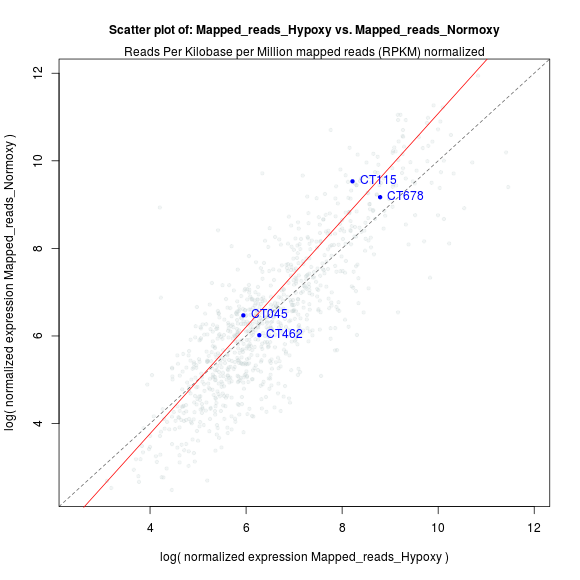
\includegraphics[width=.8\textwidth]{figure/simpleplot}
\caption{
  \textbf{Simple XY-Scatter-Plot.}
  This plot shows the simple NVT plot function result}
\label{fig:MA}
\end{figure}

\subsubsection{Advanced plot}

\begin{knitrout}
\definecolor{shadecolor}{rgb}{0.969, 0.969, 0.969}\color{fgcolor}\begin{kframe}
\begin{alltt}
\hlkwd{png}\hlstd{(}\hlkwc{filename} \hlstd{=} \hlstr{"figure/advancedplot.png"}\hlstd{,} \hlkwc{width} \hlstd{=} \hlnum{580}\hlstd{,} \hlkwc{height} \hlstd{=} \hlnum{580}\hlstd{,} \hlkwc{units} \hlstd{=} \hlstr{"px"}\hlstd{,} \hlkwc{pointsize} \hlstd{=} \hlnum{12}\hlstd{)}
\hlkwd{NVTadvancedplot}\hlstd{(mynorm,}\hlnum{2}\hlstd{,}\hlnum{2}\hlstd{,}\hlnum{4}\hlstd{)}
\hlkwd{dev.off}\hlstd{()}
\end{alltt}
\begin{verbatim}
## png 
##   2
\end{verbatim}
\end{kframe}
\end{knitrout}

\begin{figure}
\centering
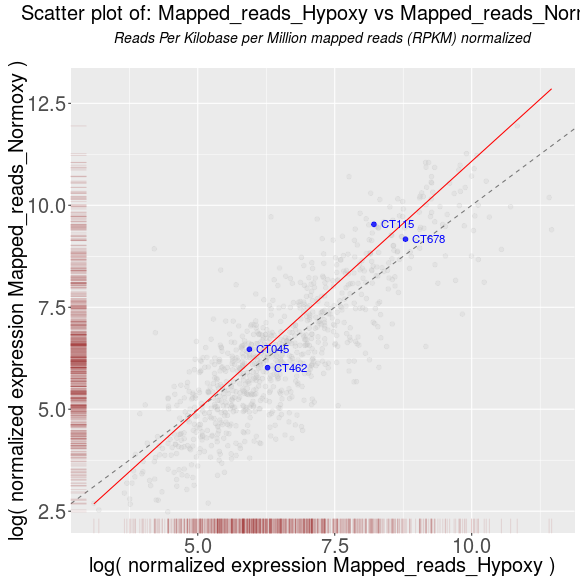
\includegraphics[width=.8\textwidth]{figure/advancedplot}
\caption{
  \textbf{Advanced XY-Scatter-Plot.}
  This plot shows the advanced NVT plot function result}
\label{fig:MA}
\end{figure}

\subsection{Correlation values}

\subsubsection{Pearson correlation}

\subsubsection{RMSD and MEA correlation}

\subsection{Test all methods}


\section{Acknowledgments}

We have benefited in the development of \nvt{} from the help and
feedback of many individuals,
\section{Session Info}

\bibliography{library}

\end{document}
